
\begin{figure}[!htbp]
\begin{center}
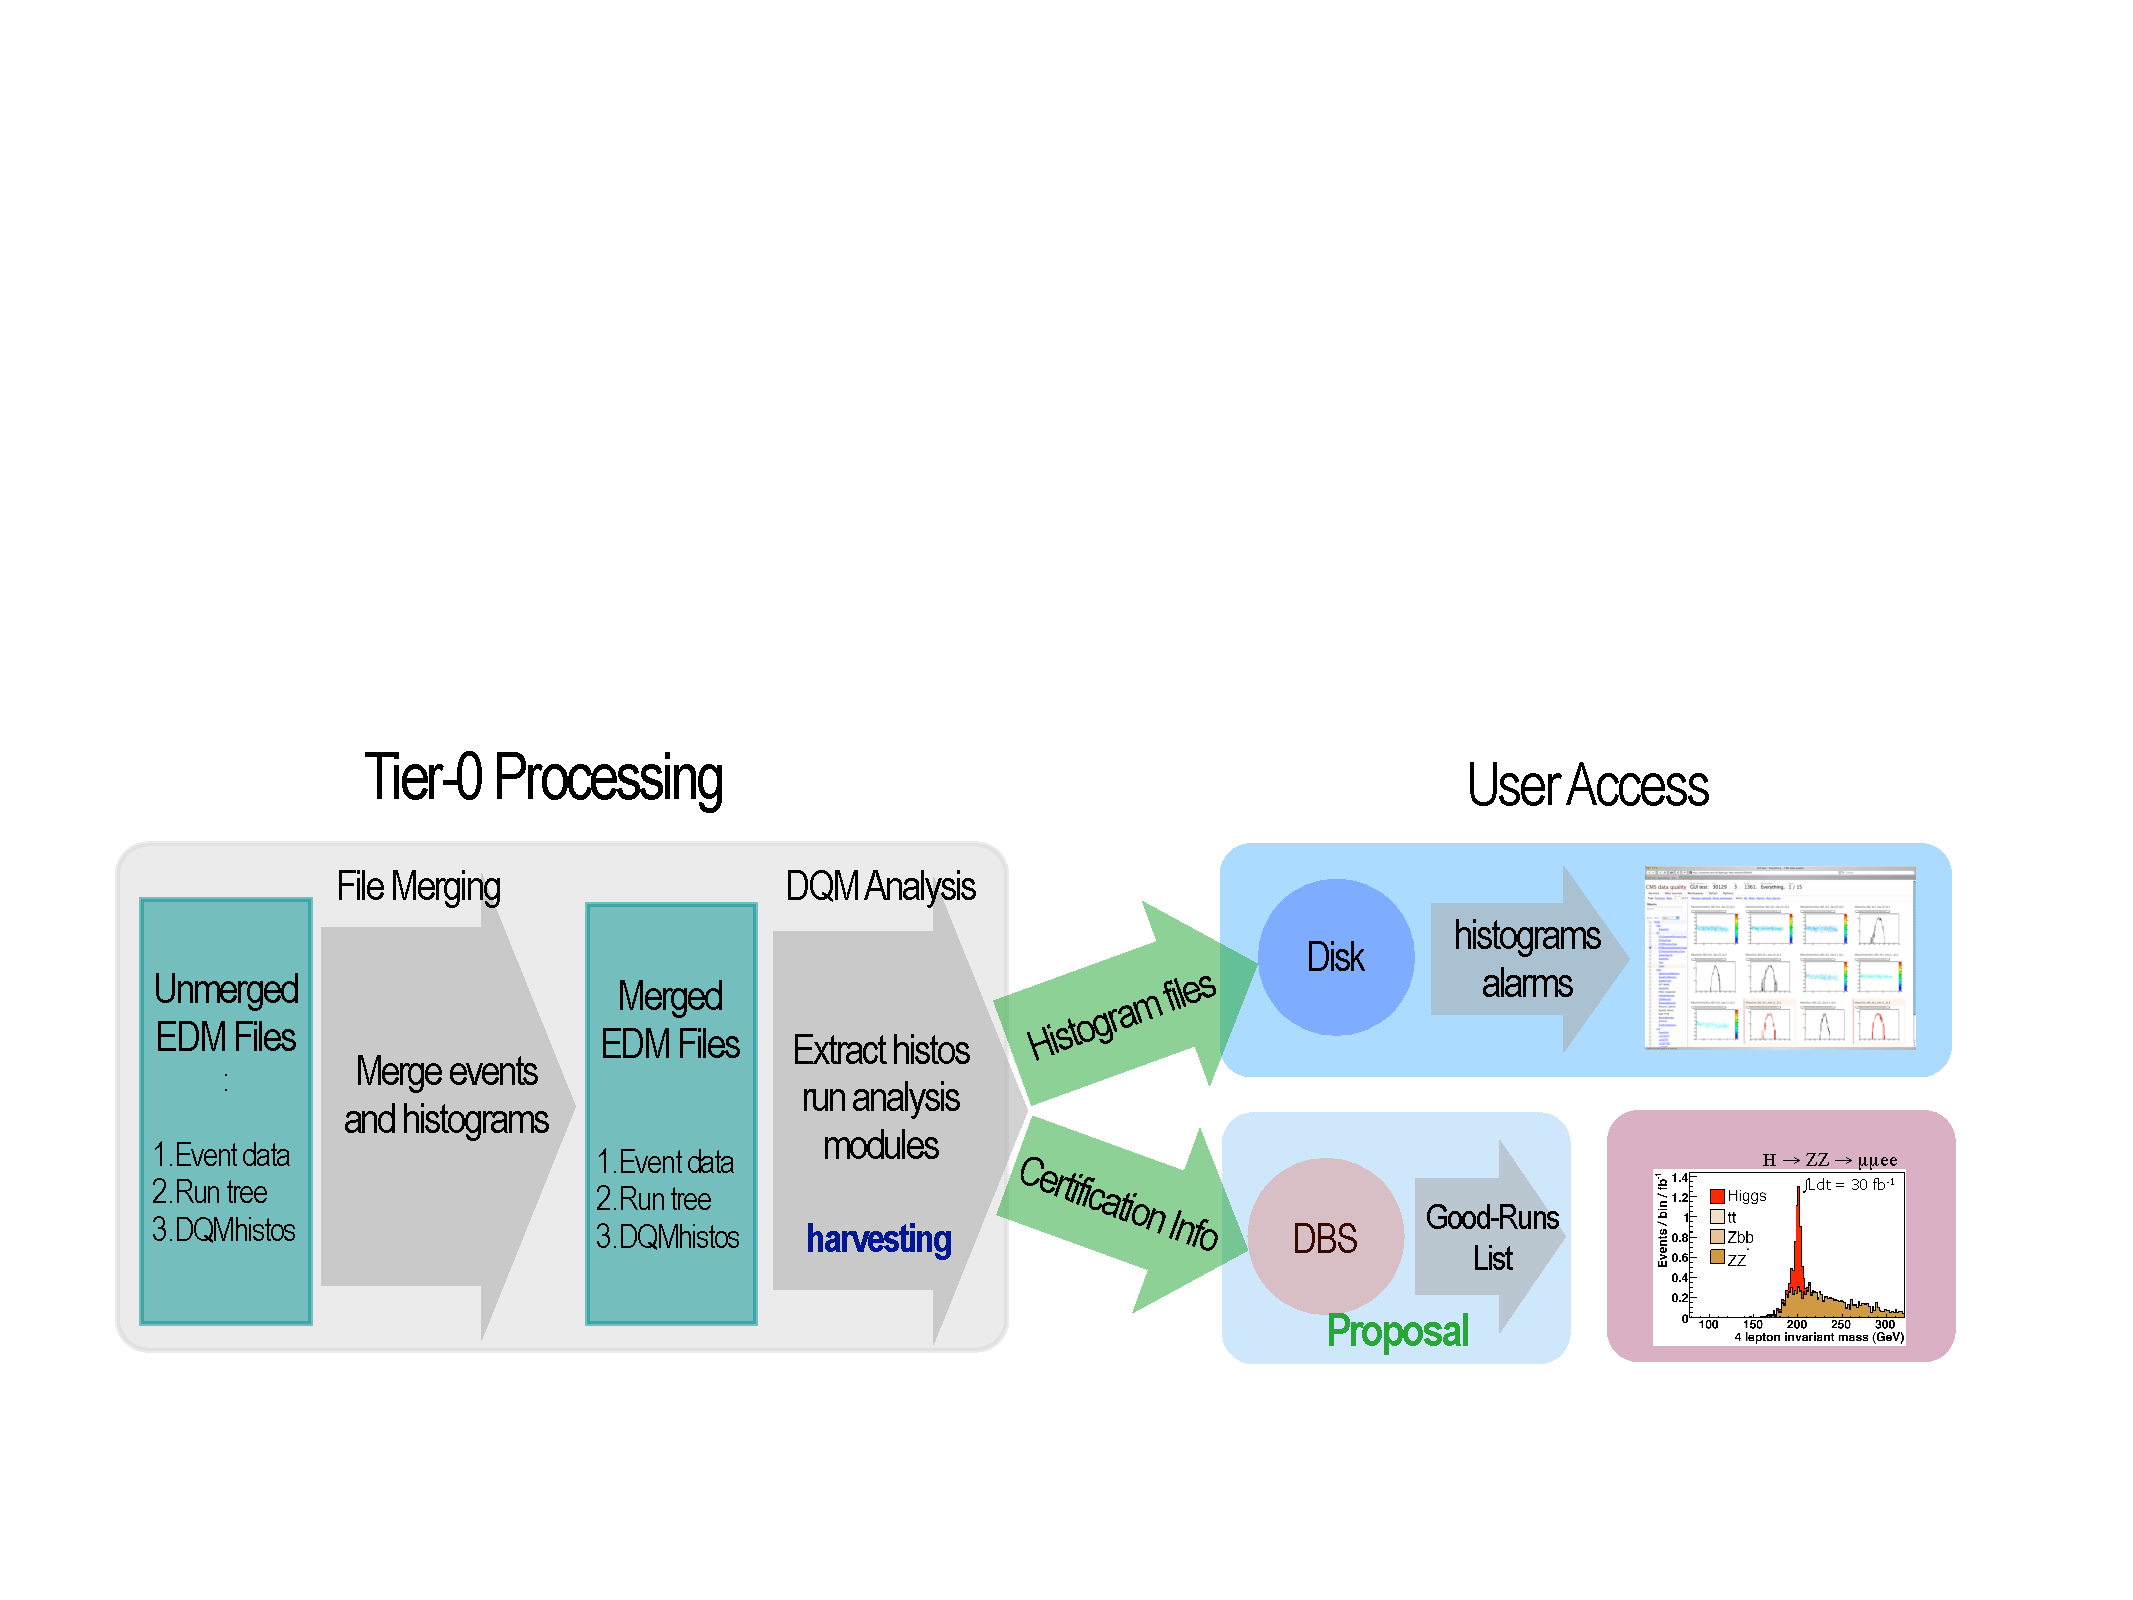
\includegraphics[width=0.9\textwidth]{dqm_tier0}
\caption{DQM data flow at Tier-0}
\end{center}
\label{fig:dqmoffline}
\end{figure}

\subsection{Prompt Reconstruction Monitoring}

Tier-0 DQM processing consists of two steps. 

\subsubsection{Histogram creation and filling}
In the first step
the histograms are created, filled with event information and stored 
in the EDM job output files (along with the processed events).
During the subsequent merging of the initially unmerged EDM files, the 
histograms are automatically summed.


\subsubsection{Harvesting step}
In a second harvesting step, the histograms are extracted from one or 
more merged EDM files, and analysis and quality test steps are performed.
Again, histograms from different files with identical names are summed up,
thus yielding the full event statistics of the dataset.

\begin{itemize}
\item{Efficiency calculation and Quality testing:\\}
These final histograms are then used as input to the calculation
of efficiencies and to quality tests.
\item{Histogram output to root-file;\\}
The output histograms and quality test results are stored in files, 
which are transfered to the file archive on the histogram DQM GUI server machine.
\item{Data certification:\\} 
Finally, the second step includes the calculation of physics data 
certification decisions. The certification information is written to the 
conditions database and into DBS. Details are described in section 
\ref{sec:certification}.
\end{itemize}

\subsection{Release Validation}

The same DQM Tier-0 infrastructure as above is used for release validation
with a few specific differences: The histograms are organized in data sets,
not per run.

\subsection{Calibration Monitoring}

\begin{figure}[!htbp]
\begin{center}
%\includegraphics[width=0.9\textwidth]{dqm_alca}
\caption{Envisaged DQM data flow for calibration and alignment purposes.}
\end{center}
\label{fig:dqmalca}
\end{figure}

The calibration workflow layout and integration will initially be performed 
on facilities at the CAF. The details are still to be defined.

\subsection{DQM at the CAF}
\label{sec:caf}

Goal: Keep DQM technology as close to Tier-0 requirements as possible,
in order to allow easy transition.
Define support of CAF activity by DQM group.
Handshake between root-file output and offline DQM GUI

%==========================================================
% this subsection is common to all sections, please fill in 
\subsection{Offline DQM Integration and Operation}

\subsubsection*{Integration}

\subsubsection*{Operation}
